\documentclass[11pt]{article}
\usepackage[margin=2.2cm]{geometry}
\usepackage[T1]{fontenc}
\usepackage{amsmath,amssymb,booktabs,graphicx,xcolor,enumitem,caption,float,siunitx}
\usepackage{hyperref}
\setlist{itemsep=2pt,topsep=3pt}
\hypersetup{colorlinks=true,linkcolor=blue!50!black,urlcolor=blue!50!black}
\captionsetup{font=small,labelfont=bf}
\setlength{\emergencystretch}{3em}
\setlength{\parskip}{4pt}
\newcommand{\fig}[2]{\begin{figure}[H]\centering\includegraphics[width=\textwidth]{figures/#1}\caption{#2}\end{figure}}
\newcommand{\figw}[3]{\begin{figure}[H]\centering\includegraphics[width=#1\textwidth]{figures/#2}\caption{#3}\end{figure}}
\newcommand{\takeaway}[1]{\par\noindent\fcolorbox{gray!50}{gray!8}{\parbox{\dimexpr\textwidth-2\fboxsep-2\fboxrule}{\textbf{Take-away.} #1}}\par\medskip}
\newcommand{\caveat}[1]{\par\noindent\fcolorbox{orange!60}{orange!6}{\parbox{\dimexpr\textwidth-2\fboxsep-2\fboxrule}{\textbf{How solid is this?} #1}}\par\medskip}
\newcommand{\novel}{\textcolor{blue!60!black}{\textbf{[new]}}}
\newcommand{\std}{\textcolor{gray}{\textbf{[standard]}}}

\title{Characterising CCD output amplifiers from their traces:\\ physics, noise origin and setup quality}
\author{ccd\_opt\_ml / amp\_phys}
\date{2026-11-16}

\begin{document}
\maketitle

\begin{abstract}
Skipper-CCD traces (0.2\,s of raw output samples) contain far more than a noise number. Combined with the readout
schematics, the process recipe and the layout, they yield an absolute calibration of the readout chain, a breakdown of
the noise into its sources, and as-built physical parameters of each amplifier and each CCD. The physical parameters
include the sense-node capacitance, the coupling capacitance of every clock line to the sense node, an implant-dose
difference between CCDs, the gate-overlap length and the buried-channel depth. The traces also give the mutual
capacitance and a shared return impedance between the video lines. Images of the same module give the thickness,
depletion, resistivity, dark charge per serial register and the crosstalk between the amplifiers. A comparison of
simultaneous images before and after a cabling change shows that the change removed most of the noise shared between
the amplifiers (correlation $0.25\to0.05$) and lowered the read noise of two amplifiers by 30\,\%. Every section explains
the physics first, then the measurement, then how solid it is. Items marked \novel{} are, as far as we know, not part of
standard CCD characterisation; \std{} items are standard and are automated here.
\end{abstract}

\tableofcontents
\newpage

% =====================================================================================================================
\section{The short version}
\begin{enumerate}
\item \textbf{Absolute calibration without a source.} A channel with no working amplifier reads the thermal (Johnson)
  noise of the frontend's load resistor, a known physical quantity. That calibrates the readout chain: $0.853\pm0.027$
  ADU/\textmu V measured, against $0.875$ by design. From it: 1.51--1.62\,\textmu V per electron at the video input,
  and the read noise in nV/$\sqrt{\text{Hz}}$ (Section~\ref{sec:cal}). \novel
\item \textbf{The output transistor is not what limits the noise.} Its thermal noise is at most 4.9\,nV/$\sqrt{\text{Hz}}$
  at 130\,K; the measured white noise is 19--22. A dead channel's trace gives the frontend alone (17.0); the live output
  stage adds $\approx$10\,nV/$\sqrt{\text{Hz}}$ on top, mostly the transistor's 1/f noise passing the CDS
  (Sections~\ref{sec:noise}, \ref{sec:traps}).
\item \textbf{The cabling change, quantified, and visible in a single trace.} The template-removed spectrum of one
  trace fell by 37--49\,\% below 1\,kHz (and 33--36\,\% from 1--100\,kHz) while the MHz floor did not move; the
  correlation of consecutive skips fell from 0.87 to 0.68--0.75. Independently, on simultaneous images: the four
  amplifiers share 20--28\,\% of their pixel noise in October and 2--7\,\% in November, and the read noise of ch0/ch1
  fell 30\,\% at the same settings (Section~\ref{sec:octnov}). \novel
\item \textbf{Every clock line's coupling to the sense node}, measured from the clock edges in the raw traces: RG
  0.15--0.37\,fF, SW 0.08--0.13, H 0.011--0.016, V $<0.003$\,fF (Section~\ref{sec:coupling}). \novel
\item \textbf{Device physics from operating data.} Sense-node capacitance $\approx$80--90\,fF; follower gain
  $\approx$0.8--0.9; buried-channel depth $\approx$0.6\,\textmu m (from the reset charge injection); a 0.85\,V
  channel-potential offset between CCDs ($\approx$0.6\,\% of the implant dose); a $\sim$0.1\,\textmu m gate overlap,
  1.7$\times$ larger on ch2 (Sections~\ref{sec:sn}--\ref{sec:knees}). \novel
\item \textbf{Each channel reads its own CCD} (the module carries four). The weak VSUB response of ch0/ch2 sits in their
  serial registers, not in the amplifiers (Section~\ref{sec:images}).
\item \textbf{Oxide traps and 1/f noise.} From how each amplifier's own noise depends on the CDS window: trap density
  $\approx2\times10^{16}$\,eV$^{-1}$cm$^{-3}$ (good oxide) on ch0/1/3, 1.5$\times$ higher on ch2 (twice the 1/f corner).
  The transistor's 1/f noise is 55--80\,\% of the single-skip noise; the 10\,\textmu s window is near-optimal and longer
  windows cost 9--32\,\% at fixed readout time (Section~\ref{sec:traps}). \novel
\item \textbf{Corrections made on the way} are listed in Section~\ref{sec:corrections}. The most important: the four
  channels' traces are separate acquisitions, so a correlation \emph{between} channels' traces is not setup noise. The
  setup noise itself is visible in each trace's spectrum; only splitting it into shared and own parts needs simultaneous
  data (images or level-1 strips).
\end{enumerate}

% =====================================================================================================================
\section{The system: what a trace is and where the signal goes}\label{sec:system}
The module PA03 carries four CCDs, each read by its own output amplifier: ch0 = CCD\_D, ch1 = CCD\_C, ch2 = CCD\_A,
ch3 = CCD\_B. They are p-channel CCDs on high-resistivity n-type silicon at 130\,K. Board 102 drives a second module, on
which three channels have no working amplifier. These \emph{dead channels} turn out to be very useful: they show what
the electronics alone does.

Figure~\ref{fig:chain} follows one electron through the chain. It is collected on the sense node (a small floating
diffusion) and changes its voltage by $q/C_{sn}$. The output transistor, a source follower, copies that voltage onto the
video line with gain $A<1$. On the frontend board the video line sees a 20\,k$\Omega$ load to ground; it is AC-coupled
(100\,nF, 100\,k$\Omega$), amplified $13.64\times2.00$ and digitised by an 18-bit ADC.
\begin{figure}[H]\centering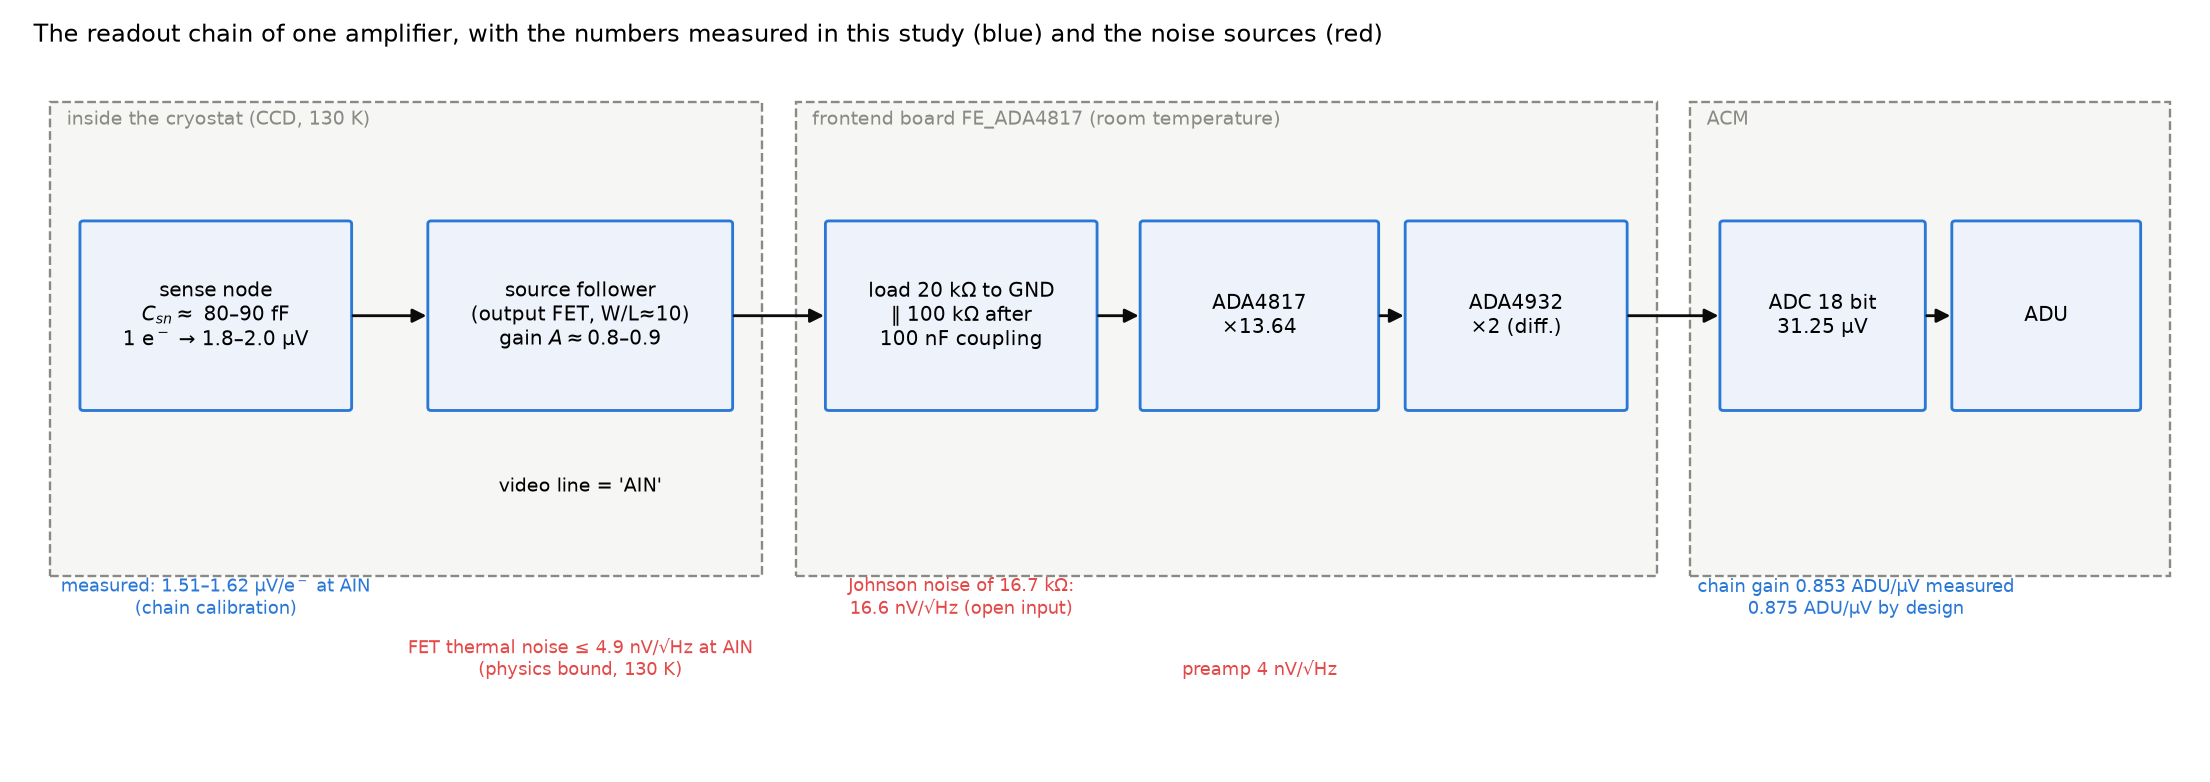
\includegraphics[width=\textwidth]{figures/readout_chain.png}
\caption{The readout chain of one amplifier, with the numbers measured in this study (blue) and the noise sources
(red).}\label{fig:chain}\end{figure}

A skipper CCD measures each pixel many times (``skips''). In every skip cycle (Figure~\ref{fig:skip}) the charge is
parked under the summing well (SW) while the sense node is reset (RG); the \emph{pedestal} is averaged for 10\,\textmu s;
the charge is moved onto the sense node; and the \emph{signal} is averaged for 10\,\textmu s. The difference (correlated
double sampling, CDS) is one measurement of the charge. A \emph{trace} records the raw samples of 10 pixels $\times$ 500
skips, plus the horizontal and vertical transfers in between, together with the sequencer's flag bits that say which
clock is switching when.
\fig{skip_cycle.png}{One skip cycle of a real trace. The CDS subtracts the pedestal window from the signal window, so
anything that sits at the same level in both windows cancels: this is why most clock couplings do not reach the image,
and why they must be measured at their edges instead (Section~\ref{sec:coupling}).\label{fig:skip}}

\paragraph{Priors used.} From the process recipe: gate dielectric 50\,nm SiO$_2$ + 50\,nm Si$_3$N$_4$ (76\,nm
oxide-equivalent, $C_{ox}=0.454$\,fF/\textmu m$^2$); buried channel B $1.3\times10^{13}$\,cm$^{-2}$ at 150\,keV. From the
frontend schematic: the load network and gains above. From the layout: output transistor $W\approx55$--60\,\textmu m,
$L\approx6$\,\textmu m; reset transistor $\approx6\times6$\,\textmu m; 15\,\textmu m pixels. From the user: 130\,K;
resistivity of order 10\,k$\Omega\cdot$cm. All in \texttt{amp\_phys/priors.toml}.

% =====================================================================================================================
\section{Electronics or CCD? The dead channels as controls}\label{sec:dead}
A dead channel goes through exactly the same readout chain as a working one; only the amplifier is missing. So anything
it shows comes from the electronics.

\paragraph{Finding the dead channels automatically.} On a channel without an amplifier the output's response to the
summing-well edge (signal-window settling) is half its normal size: 82--84\,ADU against 150--202 on every working
channel. This rule found the three dead board-102 channels, which the label fit had wrongly marked as ``ok'' with
plausible gains. \novel

\paragraph{What the electronics alone produces.}
\begin{itemize}
\item \textbf{RG feedthrough:} 70\,\% of it is board pickup (4600--4800 equivalent e$^-$/V on dead channels against
  6000--7000 on live ones).
\item \textbf{SW dip:} about half of it is board pickup.
\item \textbf{Horizontal transfers:} only 6--10\,\% pickup. The H-clock waveform is almost entirely real coupling
  through the CCD (Section~\ref{sec:coupling}).
\item \textbf{Steps and slow edges:} on board 102 these come from its electronics.
\end{itemize}
\takeaway{Before reading any ``coupling'' or ``feedthrough'' feature as a property of the CCD, subtract what a dead
channel shows. A spare unconnected channel per board is worth recording on purpose.}

% =====================================================================================================================
\section{Absolute calibration from a resistor's noise}\label{sec:cal}
A resistor at temperature $T$ produces a white voltage noise of density $\sqrt{4kTR}$; nothing about it needs to be
calibrated. A dead channel's input sees $20\,\text{k}\Omega\parallel100\,\text{k}\Omega=16.7$\,k$\Omega$ at room
temperature (16.6\,nV/$\sqrt{\text{Hz}}$) plus the preamp's 4\,nV/$\sqrt{\text{Hz}}$, i.e. 17.1\,nV/$\sqrt{\text{Hz}}$.
A CDS of two 10\,\textmu s windows turns a white density $e_n$ into $\sigma=e_n/\sqrt{\tau}=5.40$\,\textmu V per skip.
The dead channels measure 4.50--4.78\,ADU per skip, so the chain converts \textbf{0.853 $\pm$ 0.027 ADU per
\textmu V}. The schematic gives $13.64\times2.00/31.25\,\text{\textmu V} = 0.875$ (Figure~\ref{fig:cal}).
\begin{figure}[H]\centering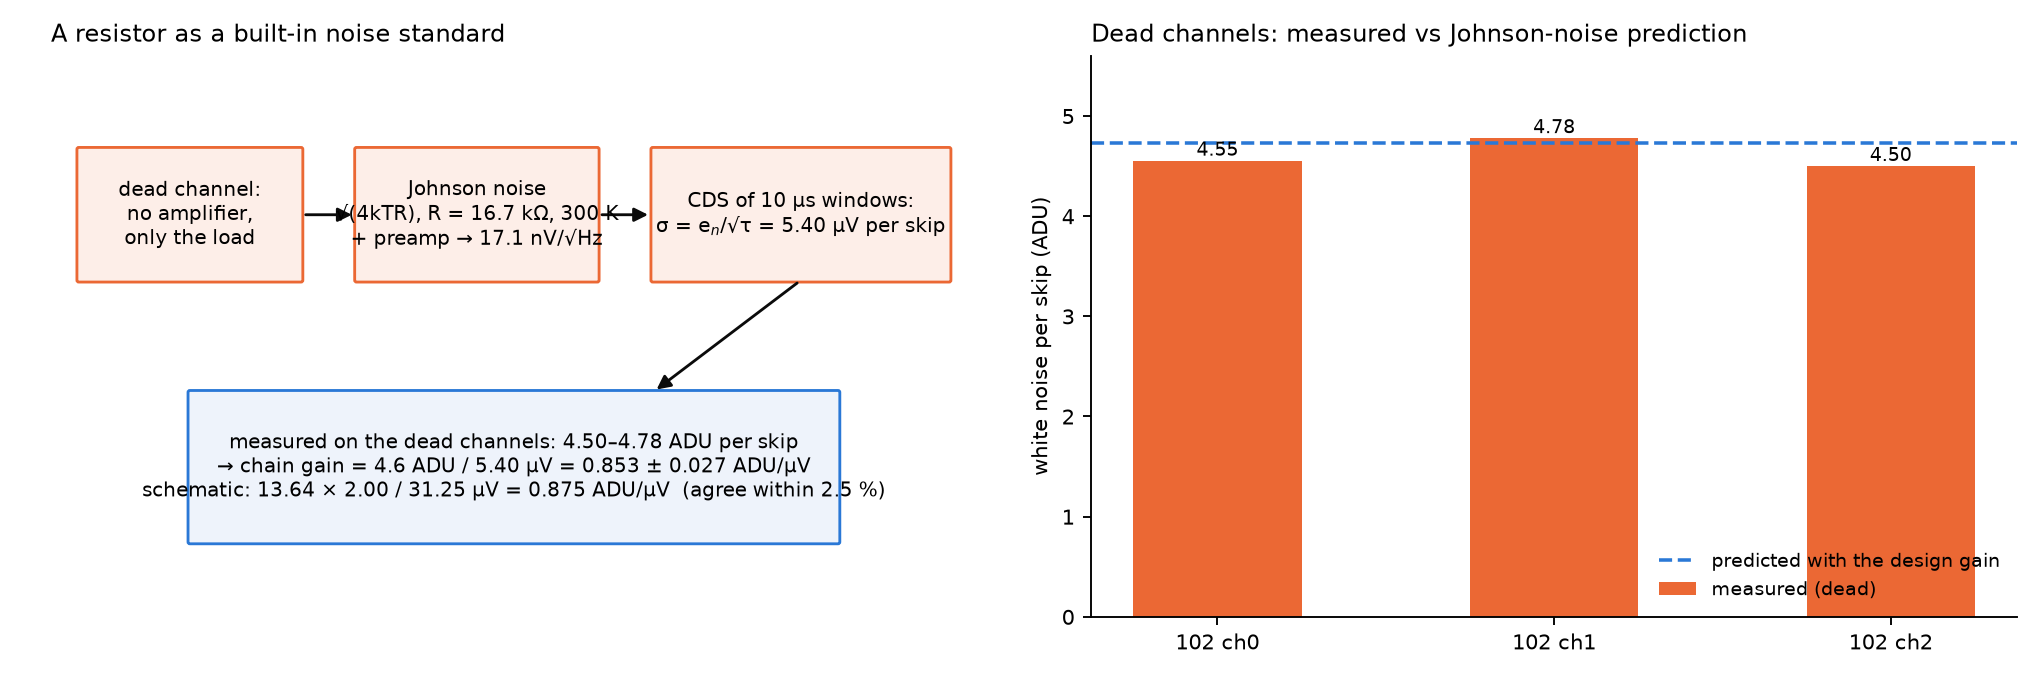
\includegraphics[width=\textwidth]{figures/dead_channel_calibration.png}
\caption{Left: the logic of the calibration. Right: the three dead channels against the prediction with the design gain.}
\label{fig:cal}\end{figure}

\paragraph{What follows from it.}
\begin{itemize}
\item \textbf{Conversion gain at the video input:} 1.62, 1.59, 1.52, 1.53\,\textmu V/e$^-$ (101 ch0--3); 1.51 for 102 ch3.
\item \textbf{White noise in physical units:} 20.2, 20.6, 21.4, 22.2\,nV/$\sqrt{\text{Hz}}$ at the video input.
\item \textbf{The ACM input buffer has unity gain} (an assumption in the design value, now checked).
\end{itemize}
\caveat{Strong: two independent routes agree within 2.5\,\%. Board 101 has no dead channel, so it uses the design value
with the 2.5\,\% as its uncertainty.}

% =====================================================================================================================
\section{What limits the noise}\label{sec:noise}
Three sources add in quadrature at the video input:
\begin{enumerate}
\item \textbf{The output transistor's channel noise}, $e_n^2=\tfrac83kT/g_m$ at the sense node, seen through the
  follower gain $A=g_mR_L/(1+g_mR_L)$. Whatever $g_m$ is, this cannot exceed 4.9\,nV/$\sqrt{\text{Hz}}$ at 130\,K with a
  20\,k$\Omega$ load: it is a small part of the measured 19--22.
\item \textbf{The load resistor and preamp}: 17.1\,nV/$\sqrt{\text{Hz}}$ on an open input. A working follower's own
  output resistance ($\approx1/g_m$) shunts the load resistor's noise; how much depends on $g_m$.
\item \textbf{Everything else}: a term the first two do not explain. The traces measure it directly: the CDS white
  noise is 19.5--19.6\,nV/$\sqrt{\text{Hz}}$ on the live amplifier and 17.0 on a dead channel (12 traces each,
  spread $\pm$0.3), so the live output stage adds $\sqrt{19.6^2-17.0^2}\approx10$\,nV/$\sqrt{\text{Hz}}$. That is the
  ``own white'' level of 9--13 found independently from the window dependence in Section~\ref{sec:traps}.
\end{enumerate}
\fig{noise_budget.png}{The white-noise budget for the two possible transistor currents. With $g_m\approx300$\,\textmu S
(favoured by the layout, Section~\ref{sec:sn}) most of the noise is the unexplained term; with $g_m\approx20$\,\textmu S
the load resistor explains most of it. One bench reading decides: the DC level of the video line (or the VDD current)
gives the transistor current and hence $g_m$.}
\takeaway{The CCD amplifiers' intrinsic \emph{thermal} noise is not the limit. Most of the ``unexplained'' term turns out
to be the output transistors' own \emph{1/f} noise, which the CDS does not remove (Section~\ref{sec:traps}). The frontend's
load network adds to it, and Section~\ref{sec:octnov} shows that the cabling matters a lot at the pixel level.}

% =====================================================================================================================
\section{The cabling change: October vs November}\label{sec:octnov}
\paragraph{First, from the trace alone.} A raw trace is a deterministic waveform (the clocks, reset and transfers,
identical every skip cycle) plus noise. Averaging all skip cycles of a trace gives the waveform (the \emph{template});
subtracting it leaves the noise, whose spectrum is the setup-plus-amplifier noise at the video input over the whole
188\,ms, at every frequency from 200\,Hz to 7.5\,MHz (Figure~\ref{fig:anat}). The dead channel, recorded the same way,
is the electronics-only reference: anything a live channel has above it comes in through the CCD, its bias and clock
lines and the cabling.
\fig{trace_anatomy_v3_ch1.png}{One trace dissected (board 101 ch1, November). Top left: the median skip cycle with the
pedestal (blue) and signal (green) windows, the summing-well dip and the reset pulse. Top right: the median horizontal
transfer. Bottom left: the noise spectrum of the whole trace once the waveform is removed. Bottom right: the quantities
extracted.\label{fig:anat}}
\fig{raw_psd_oct_nov.png}{The template-removed spectrum of one trace (101 ch1) before and after the cabling change,
with a dead channel. Left: below 20\,kHz the live channel is 10--60$\times$ above the electronics, and the cabling change
halved it. Right: above $\sim$200\,kHz the curves meet the dead channel's lines; nothing changed there.\label{fig:rawpsd}}
\begin{table}[H]\centering\small
\resizebox{\textwidth}{!}{\begin{tabular}{lcccc}\toprule
median of 12 traces & October & Nov 2--3 & Nov 10--12 & dead channel\\\midrule
spectrum 200\,Hz--1\,kHz (\textmu V/$\sqrt{\text{Hz}}$) & \textbf{67.6} & 42.8 & \textbf{34.8} & 1.6\\
spectrum 1--10\,kHz (\textmu V/$\sqrt{\text{Hz}}$) & 7.0 & 4.5 & 3.7 & 1.1\\
spectrum 10--100\,kHz (nV/$\sqrt{\text{Hz}}$) & 736 & 532 & 472 & 173\\
spectrum 0.1--1\,MHz (nV/$\sqrt{\text{Hz}}$) & 156 & 128 & 123 & 57\\
spectrum 1--7.5\,MHz (nV/$\sqrt{\text{Hz}}$) & 31.6 & 29.5 & 29.4 & 10.6\\
CDS white noise (nV/$\sqrt{\text{Hz}}$) & 20.1 & 19.5 & 19.6 & 17.0\\
correlation of consecutive skips & \textbf{0.87} & 0.75 & \textbf{0.68} & 0.26\\
variation of the noise level, 1\,ms blocks (CV) & 0.48 & 0.44 & 0.35 & 0.04\\
1\,ms blocks with bursts ($>1.5\times$ median rms) & 14\,\% & 12\,\% & 11\,\% & 0\\
excess kurtosis of the CDS & 0.00 & $-0.01$ & 0.01 & $-0.05$\\
settling time after reset / after an H transfer (\textmu s) & 0.87 / 3.14 & 0.85 / 3.14 & 0.95 / 3.16 & 1.56 / 3.01\\\bottomrule
\end{tabular}}\end{table}
\begin{itemize}
\item \textbf{The setup noise is in the trace.} Below 100\,kHz the live channel is 3--40$\times$ above the electronics,
  and that excess fell 37--49\,\% (below 1\,kHz) after the cabling change, more by Nov 10--12 than by Nov 2--3. The
  variability of the noise (bursts, block-to-block changes) fell with it.
\item \textbf{Only the low frequencies changed.} The MHz floor and the CDS white noise moved by 3--7\,\%. The change
  removed slow, low-frequency pickup, exactly the noise that 500-skip pixels average over.
\item \textbf{The skip-to-skip correlation} is a one-number summary of that slow noise as the skipper sees it: 0.87 in
  October, 0.68 now, 0.26 on the electronics alone.
\item \textbf{Settling after an H transfer is the electronics', not the CCD's} (3.0--3.2\,\textmu s on the dead channel
  too); the live output settles \emph{faster} than the dead input after reset.
\item \textbf{The noise of ch1 is Gaussian} (kurtosis 0): no single-trap telegraph noise, unlike ch2
  (Section~\ref{sec:health}).
\end{itemize}
\caveat{The October traces are longer (1.1\,s against 0.19\,s) and come from other packets; the bands above are
normalised spectra, so the length does not bias them, but small differences in window slopes or feedthrough between
the periods are not attributable to the cabling.}

\paragraph{Second, shared or own: images.} Whether that slow noise is common to the four amplifiers (the cabling, a
shared return) or each amplifier's own needs the amplifiers digitised at the same instant. The four amplifiers' traces
are \emph{separate} acquisitions, one after the other; the four amplifiers of an image (and of a level-1 strip) are read
together (Figure~\ref{fig:sim}).
\begin{figure}[H]\centering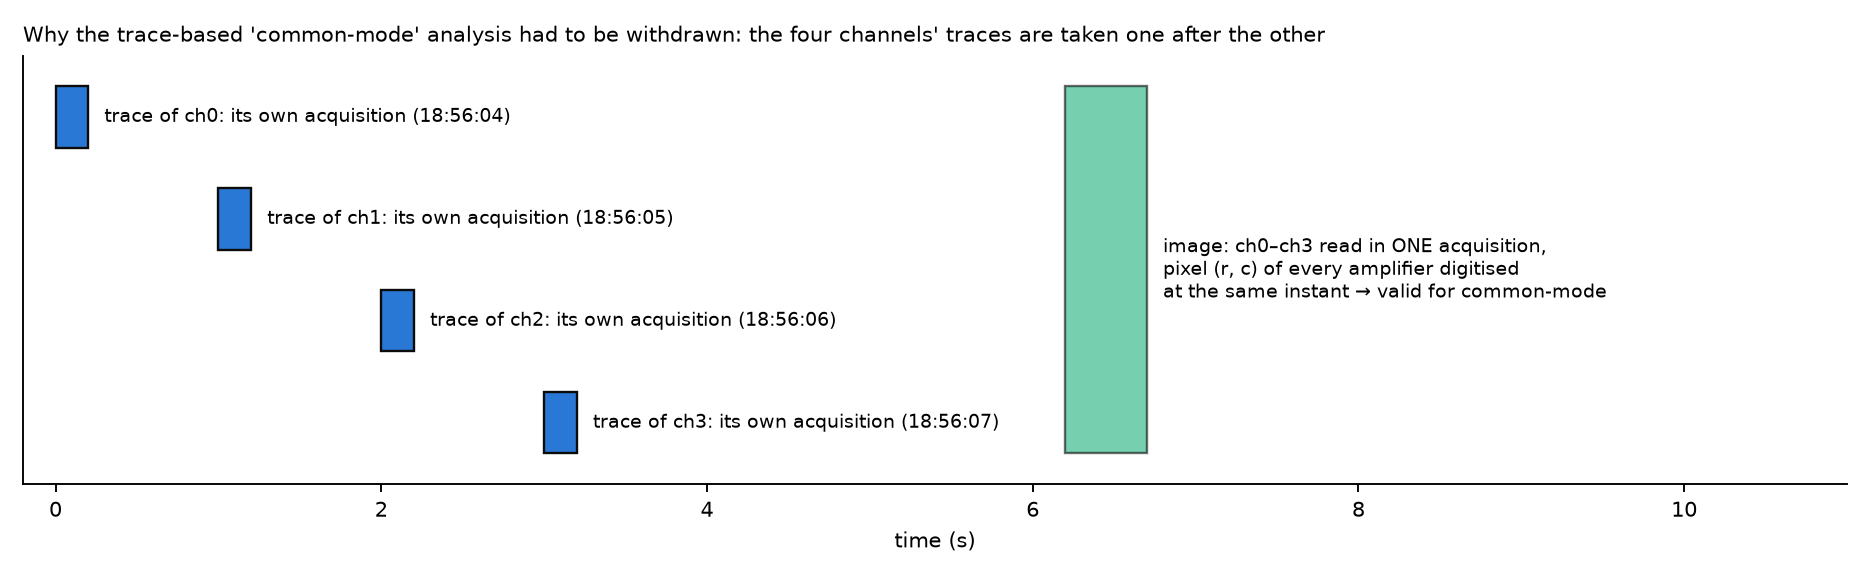
\includegraphics[width=0.9\textwidth]{figures/not_simultaneous.png}
\caption{Traces vs images: only the image is simultaneous across the amplifiers.}\label{fig:sim}\end{figure}

\paragraph{The comparison.} Board 101, 500-skip images, all at the October nominal voltages: 12 October images
against 14--25 per November period. Only pixels where every amplifier reads zero electrons are used, with the row
baseline removed (Figure~\ref{fig:octnov}).
\fig{oct_nov.png}{Before (October) and after the cabling change. Left: the 0-electron noise. Middle: the simultaneous
correlation between the amplifiers. Right: how much subtracting the common mode would help.\label{fig:octnov}}
\begin{table}[H]\centering\small
\begin{tabular}{lccc}\toprule
period & $\sigma_{0e}$ ch0 / ch1 / ch2 / ch3 (e$^-$) & correlation between amplifiers & gain from subtraction\\\midrule
October & \textbf{0.207 / 0.210} / 0.532 / 0.270 & \textbf{0.19--0.28} & \textbf{5--8\,\%}\\
Nov 2--3 & 0.154 / 0.179 / 0.517 / 0.371 & 0.03--0.06 & $\le$0.7\,\%\\
Nov 5--7 & 0.144 / 0.147 / 0.349 / 0.247 & 0.02--0.08 & $\le$0.7\,\%\\
Nov 10--12 & \textbf{0.145 / 0.148} / 0.332 / 0.291 & \textbf{0.02--0.07} & $\approx$0\,\%\\\bottomrule
\end{tabular}\end{table}
\begin{itemize}
\item \textbf{In October a quarter of the pixel noise was common to the four amplifiers.} After the change it is a few
  per cent, and subtracting it gains nothing.
\item \textbf{ch0/ch1 noise fell 30\,\%} at identical settings.
\item The per-channel white noise in the traces changed only 2--8\,\% (e.g. ch3 23.8 $\to$ 22). The change removed
  low-frequency \emph{shared} noise, which is exactly what 500-skip pixels are sensitive to.
\end{itemize}

\paragraph{Setup-quality numbers.} From \emph{one trace} of one channel: the excess of the template-removed spectrum
over the dead-channel floor at 200\,Hz--1\,kHz (October 67.6, now 34.8\,\textmu V/$\sqrt{\text{Hz}}$, electronics 1.6),
and the correlation of consecutive skips (0.87 $\to$ 0.68; electronics 0.26). Both take one trace and no charge. From a
simultaneous image or strip: $\rho_\text{sim}$, the mean correlation of zero-electron pixels between the amplifiers,
row baseline removed (October 0.25, November 0.05, target 0), which says how much of the remainder is shared. \novel
\caveat{Solid for ch0/ch1. ch2/ch3 scatter more (ch2 has its own problem). The October images had longer exposures
(10--100\,s), but that adds $\le$0.1\,e$^-$/pixel and the zero-electron selection excludes it.}

% =====================================================================================================================
\section{How each clock line couples to the sense node}\label{sec:coupling}
Every gate overlaps the silicon near the sense node a little, so a voltage step $\Delta V$ on that line pushes a charge
$C_k\,\Delta V$ onto the node. In the CDS these steps cancel (Figure~\ref{fig:skip}), so they must be measured at the
edges. The trace flags mark every horizontal (bit 6) and vertical (bit 7) transfer, so the raw samples around each edge
can be averaged and the jump at the edge measured. In the v3 data every rail's high and low level was varied over 80
settings. Regressing each edge's jump on all rails at once tells which line causes it and how strongly, in ADU per volt.
Divided by the gain and multiplied by $q$, that is the coupling capacitance (Figure~\ref{fig:edges}).
\fig{clock_edges.png}{The average horizontal-transfer waveform. The board-101 channels swing by $\pm$40\,000\,ADU, the dead
board-102 channels (grey) by a few thousand: the H response is real coupling through the CCD amplifier, not pickup. The
numbered edges are those analysed.\label{fig:edges}}
\fig{coupling_bars.png}{Every line's coupling to the sense node: measured (blue), upper limit (grey), estimated from the
layout (orange). For scale, the sense node itself is $\approx$85\,fF.}
\begin{table}[H]\centering\small
\begin{tabular}{lll}\toprule
line & coupling to the sense node & how\\\midrule
RG (reset gate) & 0.15--0.37\,fF (ch2 highest) & edges + feedthrough, pickup subtracted\\
SW (summing well) & 0.08--0.13\,fF & skip-cycle feedthrough\\
H1, H2, H3 & 0.011--0.016\,fF & H-transfer edges, $z>4$ on all four amplifiers\\
V1, V2, V3 & $<$0.002--0.003\,fF & V-transfer edges (not detected)\\
OG & $\sim$0.2--0.6\,fF (estimate) & not varied in v3\\
VDD / drain & $\sim$2--4\,fF (estimate) & output-FET gate--drain overlap\\
VSUB & $\sim$0.01--0.03\,fF (estimate) & sense-node area / depleted silicon\\\bottomrule
\end{tabular}\end{table}
\paragraph{Why it matters for noise.} A noise $v_n$ on line $k$ appears on the sense node as $v_nC_k/C_{sn}$. To
inject 22\,nV/$\sqrt{\text{Hz}}$, VDD would need only 0.6\,\textmu V/$\sqrt{\text{Hz}}$; OG 5; RG 7; SW 19; VSUB
$\sim$60; H $\sim$190. VDD is the line that must be quietest. \novel
\caveat{The H couplings are clear (significant on all four amplifiers). The V limits are solid. OG, VDD and VSUB are
estimates: they need a dither measurement (Section~\ref{sec:next}).}

% =====================================================================================================================
\section{Inside the sense node: capacitance and follower gain}\label{sec:sn}
The measured 1.56\,\textmu V/e$^-$ at the video input is $A\,q/C_{sn}$: two unknowns. The layout adds a third relation.
In a source follower the gate--source capacitance $C_{gs}\approx\tfrac23C_{ox}WL\approx105$\,fF is \emph{bootstrapped}:
its source follows the gate, so only $(1-A)$ of it loads the node:
\begin{equation}C_{sn}=C_\text{fixed}+C_{gs}(1-A),\end{equation}
where $C_\text{fixed}$ collects the diffusion, the overlaps and the $\sim$100\,\textmu m sense line. Device physics for
this transistor ($W/L\approx10$, buried p-channel at 130\,K, 100--250\,\textmu A through the 20\,k$\Omega$ load) gives
$g_m\approx170$--750\,\textmu S, i.e. $A\approx0.77$--0.94. The two routes cross (Figure~\ref{fig:boot}):
\fig{bootstrap.png}{Left: the follower gain the measured conversion gain requires, for each value of the fixed
capacitance (blue), against the device-physics range (orange). Right: the resulting sense-node capacitance.\label{fig:boot}}
\begin{itemize}
\item $A\approx0.8$--0.9, $g_m\approx200$--400\,\textmu S;
\item $C_{sn}\approx80$--90\,fF, i.e. $\approx$1.8--2.0\,\textmu V per electron at the sense node;
\item $C_\text{fixed}\approx60$--80\,fF: most of the node capacitance is wiring and diffusion, not the gate. A shorter
  sense line would raise the conversion gain. \novel
\end{itemize}
\caveat{Model-dependent. The DC level of the video line (one voltmeter reading) gives the transistor current and settles
$g_m$, $A$ and $C_{sn}$ per amplifier.}

% =====================================================================================================================
\section{The buried-channel depth from the reset charge injection}\label{sec:depth}
\paragraph{Buried channel.} In these CCDs a boron implant makes the potential maximum for the holes \emph{inside} the
silicon, at a depth $x_{ch}$ below the oxide (Figure~\ref{fig:bc}, left). This keeps the charge away from the traps at the
oxide surface. The gate therefore couples to the channel charge through two capacitances in series: the dielectric and
the silicon above the channel (Figure~\ref{fig:bc}, right):
\begin{equation}\frac1{C_\text{eff}}=\frac{t_{eq}}{\varepsilon_{ox}}+\frac{x_{ch}}{\varepsilon_{Si}}.\end{equation}
\fig{buried_channel.png}{Left: cross-section of a gate on the buried channel (not to scale; the potential profile is
schematic). Right: the series capacitances through which the gate sees the channel charge.\label{fig:bc}}

\paragraph{Charge injection.} When RG switches the reset transistor off, the charge in its channel,
$Q=C_\text{eff}WL\,(V_\text{overdrive})$, leaves through both ends, roughly half onto the sense node
(Figure~\ref{fig:inj}, left). The overdrive is set by RG$_\text{high}-$VR. Indeed, the measured reset jump depends on RG$_\text{high}$
and VR with equal and opposite coefficients, i.e. on RG$_\text{high}-$VR only, rising by \textbf{2.1--2.4\,fF per volt}
on all four CCDs (Figure~\ref{fig:inj}, right).
\fig{charge_injection.png}{Left: what happens at reset. Right: the measured jump (as charge on the sense node) against
RG$_\text{high}-$VR over the 80 v3 settings.\label{fig:inj}}

\paragraph{From the slope to the depth.}
\begin{itemize}
\item $\tfrac12C_\text{eff}\times36\,\text{\textmu m}^2=2.25$\,fF $\Rightarrow C_\text{eff}\approx0.125$\,fF/\textmu m$^2$.
\item With the recipe's 76\,nm oxide-equivalent ($C_{ox}=0.454$), the silicon part is $1/(1/0.125-1/0.454)=0.172$\,fF/\textmu m$^2$,
  so $x_{ch}=\varepsilon_{Si}/0.172\approx$ \textbf{0.6\,\textmu m}.
\item Check: boron at 150\,keV has a projected range of $\approx$0.45\,\textmu m (straggle 0.1\,\textmu m), deepened by
  the later oxidations and anneals. 0.5--0.7\,\textmu m is what the process should give. \novel
\end{itemize}
\paragraph{Oxide thickness: what can and cannot be separated.} Every electrical handle (this injection, the knees of
Section~\ref{sec:knees}, the output-FET gate capacitance) measures the \emph{combination} $t_{eq}/\varepsilon_{ox}+x_{ch}/\varepsilon_{Si}
\approx8.0$\,\textmu m$^2$/fF. Assuming $t_{eq}=76$\,nm gives $x_{ch}\approx0.6$\,\textmu m. Assuming $x_{ch}=0.45$\,\textmu m
gives $t_{eq}\approx126$\,nm. The recipe pair is self-consistent. To measure the oxide alone, measure the capacitance of
a clock line at the connector: a V phase covers a third of the array, so $C_\text{line}=\varepsilon_{ox}A/t_{eq}$ is
0.1--0.3\,\textmu F and easy to measure. Then the depth follows per CCD.
\caveat{Model-dependent: the ``half'' split is an assumption (30--70\,\% gives 0.3--0.9\,\textmu m), and the gate area is
read from the layout ($\pm$10\,\%). Slowing the RG edge with an RC would pin the split.}

% =====================================================================================================================
\section{Channel potentials and implant dose: the knees}\label{sec:knees}
As a clock rail is moved across its window, at some voltage a barrier or well under that gate is crossed: transfer
starts to fail, reset loses headroom, a surface inverts. The outputs then change slope: a ``knee''. Hinge fits (a line
with a break), with all other 17 rails regressed out, find these knees per CCD (Figures~\ref{fig:kc} and \ref{fig:kd}).
\figw{0.75}{knees_concept.png}{Schematic of a knee and the 0.85\,V shift found for CCD\_B on the H3 low rail.\label{fig:kc}}
\fig{knees.png}{Measured knees: $\lambda$ against VSUB (left) and $\sigma_e$ against VR (right), with the other voltages
regressed out.\label{fig:kd}}
\begin{itemize}
\item \textbf{H3 low rail:} 6.2--6.45\,V on CCD\_D and CCD\_C, \textbf{5.35--5.55\,V on CCD\_B}. In a buried channel the
  potential shifts by $\Delta V\approx q\,\Delta N_s/C_\text{eff}$, so 0.85\,V $\approx8\times10^{10}$\,cm$^{-2}$ $\approx$
  \textbf{0.6\,\% of the implant dose} (or the same amount of fixed oxide charge). \novel
\item \textbf{VR (reset headroom):} $-2.5$ to $-3.8$\,V. ch0's noise starts rising at a less negative VR than the others.
\item \textbf{VSUB ($\lambda$):} 54--57\,V on all CCDs. This is \emph{not} depletion (Section~\ref{sec:images}).
\end{itemize}
\caveat{The v3 design moves every rail at once, which blurs the knees ($\pm$0.2--0.4\,V). Stepping one rail at a time
gives $\pm$0.05\,V.}

% =====================================================================================================================
\section{Oxide traps and the transistor's 1/f noise}\label{sec:traps}
\paragraph{The physics.} The gate oxide of the output transistor contains traps. Carriers in the channel tunnel into
them and back out, each with its own time constant; the sum over many traps with a broad spread of time constants is
1/f noise. In the McWhorter number-fluctuation model the gate-referred noise is
\begin{equation}S_{V_g}(f)=\frac{q^2kT\lambda N_t}{WL\,C^2\,f}
\quad\Longrightarrow\quad N_t=\frac{K_{V_g}\,WL\,C^2}{q^2kT\lambda},\end{equation}
where $K_{V_g}=S_{V_g}f$ is the 1/f coefficient at the gate (= the sense node), $WL\approx345$\,\textmu m$^2$ (layout),
$C$ the gate capacitance per area, $T=130$\,K and $\lambda\approx0.1$\,nm the tunnelling attenuation length. $N_t$ is the
trap density per energy and volume: about $10^{16}$--$10^{17}$\,eV$^{-1}$cm$^{-3}$ for good thermal oxide, $\sim10^{18}$
for poor oxide.

\paragraph{Why the noise-vs-skips curve cannot measure it.} The CDS subtracts two windows 13.8\,\textmu s apart. That
suppresses low frequencies as $f^2$, so what is left of the 1/f noise sits at 10--40\,kHz, close to the skip rate
(Figure~\ref{fig:cdsT}, left). Averaging skips then reduces it almost exactly like white noise (right). A first attempt
that tried to read the 1/f level from how the noise falls with more skips therefore failed: the two shapes are almost the
same.
\fig{cds_transfer.png}{Left: the CDS filter and what white and 1/f noise look like after it. Right: the noise of an
average of $N$ skips, for white and for 1/f noise at the input: both fall as $1/\sqrt N$.\label{fig:cdsT}}

\paragraph{The handle that works: the window length.} White noise in a CDS falls as $1/\sqrt\tau$ with the window length
$\tau$; the 1/f part is almost independent of $\tau$. The v2 data varied the window from 3 to 30\,\textmu s, and every v2
packet has a level-1 strip at its own settings, with all channels recorded simultaneously. For each amplifier:
\begin{enumerate}
\item take its per-skip values and subtract the part shared with the other channels (the setup), leaving its \emph{own}
  noise;
\item measure the single-skip noise $\sigma_1$ in each of the 100 strips;
\item fit $\sigma_1^2(\tau)=S_wI_w(\tau)+K\,I_f(\tau)$, where $I_w$ and $I_f$ are the white and 1/f noise integrated
  through the \emph{exact} filter of each setting: CDS windows $\tau$, centres $\tau+3.8$\,\textmu s apart, the skip
  period growing with $\tau$, and the consecutive-skip difference used to remove the pixel charge.
\end{enumerate}
\fig{oxide_traps_tau.png}{Single-skip noise against the CDS window over the 100 v2 strips. Left: each amplifier's own
noise, with the white + 1/f fits; they describe the data closely. Right: the total noise. It turns back \emph{up} above
$\sim$15\,\textmu s: the shared (setup) slow noise leaks in more as the windows get longer.\label{fig:otau}}

\paragraph{Results.}
\begin{table}[H]\centering\small
\begin{tabular}{lcccc}\toprule
 & ch0 & ch1 & ch2 & ch3\\\midrule
own white noise at the video input (nV/$\sqrt{\text{Hz}}$) & 10.2 & 10.4 & 8.7 & 13.1\\
1/f corner frequency & 52\,kHz & 51\,kHz & \textbf{106\,kHz} & 34\,kHz\\
1/f share of the single-skip noise (10\,\textmu s window) & 66\,\% & 66\,\% & \textbf{80\,\%} & 56\,\%\\
$N_t$, $A=0.85$, $C=C_{ox}$ (eV$^{-1}$cm$^{-3}$) & $1.9\times10^{16}$ & $1.9\times10^{16}$ & $\mathbf{2.8\times10^{16}}$ & $2.0\times10^{16}$\\
$N_t$, $A=0.44$, $C=C_{ox}$ & $7.0\times10^{16}$ & $7.0\times10^{16}$ & $1.0\times10^{17}$ & $7.5\times10^{16}$\\
$N_t$, $A=0.85$, $C=C_\text{eff}$ (buried channel) & $1.4\times10^{15}$ & $1.4\times10^{15}$ & $2.1\times10^{15}$ & $1.5\times10^{15}$\\\bottomrule
\end{tabular}\end{table}
\begin{itemize}
\item \textbf{The oxides are good.} All four amplifiers sit in the range of good thermal oxide. No output transistor has
  a damaged or contaminated gate oxide.
\item \textbf{ch2 is worse, for a physical reason.} It has $\sim$1.5$\times$ the trap density and twice the 1/f corner.
  That fits its telegraph noise, its higher noise floor and its least stable noise: the amplifier excluded since v1 has a
  gate oxide with more traps, including at least one large single trap. \novel
\item \textbf{Most of each amplifier's single-skip noise is 1/f.} Its own white noise is only 9--13\,nV/$\sqrt{\text{Hz}}$;
  the 1/f part is 55--80\,\% of the variance. This is most of the ``unexplained'' term of Section~\ref{sec:noise}: the
  transistors' own 1/f noise passing through the CDS, not setup injection.
\item \textbf{The skipper noise floor is not this 1/f.} The excess at long averaging (at 240 skips the total noise is
  2.4$\times$ white, the own noise 1.3$\times$) comes from slower, steeper-spectrum wander, mostly shared between the
  channels: the setup (Section~\ref{sec:octnov}).
\end{itemize}

\paragraph{A practical rule: the optimal window.} For a fixed readout time, a longer window means fewer skips. With the
fitted white and 1/f levels, the noise at fixed time is lowest for 5--8\,\textmu s windows (Figure~\ref{fig:wopt}). The
present 10\,\textmu s is within 1--5\,\% of that optimum. Longer windows cost 9--32\,\% at the same total time, because the
1/f part does not shrink while the number of skips does. Including the shared slow noise, which grows with the window
(Figure~\ref{fig:otau}, right), long windows are even worse.
\fig{window_optimum.png}{Left: each amplifier's single-skip noise against the window, split into white (dashed) and 1/f
(dotted). Right: the noise reached in a fixed readout time, relative to the present 10\,\textmu s window.\label{fig:wopt}}
\takeaway{Spend a fixed image time on more skips, not on longer CDS windows. 5--10\,\textmu s windows are optimal for these
amplifiers.}
\caveat{The comparison between amplifiers (ch2 worst), the 1/f share and the optimal window are robust. The absolute
$N_t$ depends on two choices: the follower gain (0.44 instead of 0.85 makes it $\sim$3.7$\times$ higher, still good) and
whether the traps couple through the oxide capacitance or the buried-channel coupling ($\sim$13$\times$ lower), plus the
standard $\lambda$. They are upper limits: any own slow noise that is not the transistor's 1/f also counts. The DC level
of the video line, which settles the follower gain, firms up the scale.}

% =====================================================================================================================
\section{Between the channels: crosstalk, video-line capacitance, shared return}\label{sec:xtalk}
When one amplifier reads a large charge (a track), a tiny fraction appears on the others at the same instant:
$\sim10^{-4}$, so a $10^4$\,e$^-$ track makes $\pm1$\,e$^-$ ghosts. Two mechanisms can cause it. They are separated by
how the crosstalk depends on the CDS window $\tau$ (Figure~\ref{fig:xt}):
\begin{itemize}
\item \textbf{Capacitance between the video lines} injects a short pulse, which the window averages: crosstalk $\propto
  1/\tau$, with $C_m=a/R_\text{out}$.
\item \textbf{A shared return impedance} shifts the other channel's reference by the opposite amount, independent of
  $\tau$: crosstalk $=-Z/R_L$.
\end{itemize}
\fig{crosstalk_window.png}{Crosstalk against $1/\tau$ (v2 images at three window lengths). Left: the positive pairs fall
with longer windows, i.e. capacitance between video lines. Right: the ch0$\leftrightarrow$ch2 and ch1$\leftrightarrow$ch3
pairs keep a negative, window-independent part, i.e. a shared return.\label{fig:xt}}
\begin{itemize}
\item \textbf{Video-line mutual capacitance:} 0.1--0.85\,pF per pair; largest for the neighbouring pairs ch0--ch1 and
  ch2--ch3. \novel
\item \textbf{Shared return:} $\approx$2--4\,$\Omega$ between ch0/ch2 and ch1/ch3: a specific grounding item to fix. \novel
\item \textbf{Inside the package:} no positive window-independent part, so the CCDs do not couple at the sense nodes
  ($\lesssim0.01$\,fF).
\end{itemize}

% =====================================================================================================================
\section{The silicon: what the images add}\label{sec:images}
Images of the same module (October runs) give what traces cannot. \std{} methods, with the per-CCD results:
\begin{itemize}
\item \textbf{Gain from single-electron peaks} (Figure~\ref{fig:peaks}): 1.25--1.32\,ADU/e$^-$, 6\,\% below November on
  all amplifiers alike: a common change of the readout scale, consistent with the readout change.
\item \textbf{Noise against the number of skips} (Figure~\ref{fig:nvs}): white down to a floor of $\approx$0.1\,e$^-$
  (0.2 on ch2).
\item \textbf{Thickness from muons} (Figure~\ref{fig:tracks}): 615--655\,\textmu m. \textbf{Diffusion} from the track
  width, front to back: 0.25 $\to$ 1.4 pixels: fully depleted, field-free layer $\lesssim$50\,\textmu m.
\end{itemize}
\fig{peaks_101.png}{Single-electron peaks in the skipper images: the spacing is the gain.\label{fig:peaks}}
\fig{noise_vs_skips.png}{Noise against the number of skips: $1/\sqrt{N}$, then a floor.\label{fig:nvs}}
\fig{tracks_Q_vs_L.png}{Muon tracks: charge against projected length; the fit gives the thickness.\label{fig:tracks}}
\fig{tracks_diffusion_thickness.png}{Track width (diffusion) against depth.}

\paragraph{Resistivity.} Full depletion of 615--655\,\textmu m at VSUB $\le$ 45--55\,V requires
$\rho\gtrsim$ \textbf{25--35\,k$\Omega\cdot$cm} (Figure~\ref{fig:dep}). The $\lambda$ knee at 54--57\,V lies above full
depletion, so it is something else: a serial-register effect. \novel
\fig{depletion.png}{Depletion depth against VSUB for several resistivities, with the measured thickness. Full depletion
at the nominal 45\,V needs $\rho\gtrsim$25--35\,k$\Omega\cdot$cm.\label{fig:dep}}

\paragraph{Dark charge per CCD and the ch0/ch2 puzzle.} With all 18 voltages regressed out, the weak VSUB response of
ch0 and ch2 sits entirely in the \emph{serial-register} dark charge and the overscan (+2.0 and +0.8\,\%/V against +7.5
and +5.8\,\%/V); the array dark charge shows no such pairing (Figure~\ref{fig:dark}). Since each channel reads its own
CCD, this is a property of each CCD's serial register, not of the amplifier.
\fig{dark_vs_vsub.png}{Dark charge against VSUB, array and serial register separately, per CCD.\label{fig:dark}}
\fig{defects_profiles.png}{Defect profiles: hot columns and a localised emitter on CCD\_B, glow at the amplifier end of
ch2's register.}
\fig{pp_dipoles.png}{Pocket pumping: on board 101 an artefact of the pump clocking hides the trap dipoles; on board 102
pumpable traps are below $\sim10^{-3}$ per pixel.}

% =====================================================================================================================
\section{Simple physics equations instead of machine learning}\label{sec:eq}
Each equation was fitted on three board-101 amplifiers and tested on the fourth:
\begin{itemize}
\item \textbf{Gain:} $\ln g=\ln g_0+b\,\Delta\text{VDD}+c\,\Delta\text{VR}+d\,\Delta\text{VR}^2$.
\item \textbf{Dark charge:} $\ln\lambda=\ln\lambda_0+\beta\,\Delta\text{VSUB}+\gamma(\text{VSUB}-56)_++\sum b_k\Delta V_k$.
\item \textbf{Noise:} $\sigma_e=\sqrt{s^2\sigma_\text{trace}^2+\kappa\lambda g^2}/g$.
\end{itemize}
\fig{physics_model.png}{Each amplifier predicted from the other three plus one nominal image of its own.}
\begin{table}[H]\centering\small
\begin{tabular}{llll}\toprule
target & physics, no image & physics, one image & best machine learning (new amplifier)\\\midrule
gain & 3.5\,\% (3 constants) & 3.8\,\% & 3.7\,\%\\
dark charge & 57\,\% & \textbf{32\,\%} & 40\,\%\\
noise & 20\,\% (9--14\,\% on ch0/ch1) & 19\,\% & 11.9\,\%\\\bottomrule
\end{tabular}\end{table}
\begin{itemize}
\item \textbf{Gain:} three constants match machine learning. The VDD slope ($-1.6\,\%$/V) is universal.
\item \textbf{Dark charge:} one image of a new CCD plus the shared slopes beats every model without that image. No trace
  can know a different CCD's dark charge.
\item \textbf{Noise:} the equation fails exactly on the two amplifiers with anomalous slow noise (ch2 telegraph, ch3
  excess). The failure is itself a health flag.
\end{itemize}

% =====================================================================================================================
\section{Amplifier health at a glance}\label{sec:health}
Each amplifier's quantities are compared with the others in units of their combined error; $|z|>3$ marks an outlier
(Figure~\ref{fig:out}).
\fig{outliers.png}{How far each amplifier sits from the others, per quantity. 101 ch2 stands out for telegraph noise
(excess kurtosis $z=+4.5$, jump share, steeper 1/f); 102 ch3 differs in many electronics quantities, most of which its
dead neighbours share (board-102 electronics).\label{fig:out}}
\begin{itemize}
\item \textbf{101 ch2}, excluded since v1: a charge trap in its output transistor (telegraph noise), 2$\times$ the noise
  floor, the largest RG overlap and glow at the amplifier end of its register. Everything points to its output stage.
\item \textbf{101 ch3:} excess slow noise (Allan deviation $z=+4.3$).
\item \textbf{102 ch3:} settles like a working amplifier but sees no charge (images and H transfers). The channel mapping
  between traces and images on board 102 is to be checked.
\end{itemize}

% =====================================================================================================================
\section{What is new, and how solid it is}\label{sec:new}
\begin{table}[H]\centering\small
\begin{tabular}{p{6.2cm}p{2.2cm}p{6.6cm}}\toprule
quantity & status & what limits it\\\midrule
chain gain from Johnson noise & \novel{} solid & board 101 uses the design value ($\pm$2.5\,\%)\\
dead-channel separation of pickup & \novel{} solid & assumes equal pickup on both boards\\
setup number $\rho_\text{sim}$ (October/November) & \novel{} solid & one image per check today\\
clock $\to$ sense-node couplings (RG, SW, H, V) & \novel{} solid & OG, DG, TG, VDD, VSUB only estimated\\
crosstalk matrix & \std{} solid & --\\
video-line capacitance, shared return & \novel{} indicative & 30--100\,\% errors; three window groups\\
$C_{sn}$, $A$, $g_m$ & \novel{} model & one DC reading decides\\
gate overlap under RG & \novel{} model & scales with the oxide thickness\\
buried-channel depth & \novel{} model & charge split, gate area; oxide degeneracy\\
setup noise from one trace (spectrum excess, skip correlation) & \novel{} solid & needs a dead-channel reference\\
output-stage noise = live $-$ dead in quadrature ($\approx$10\,nV/$\sqrt{\text{Hz}}$) & \novel{} solid & assumes the same frontend\\
oxide trap density, 1/f corner per amplifier & \novel{} solid relative, model absolute & follower gain, $C$ choice; upper limit\\
optimal CDS window (5--10\,\textmu s) & \novel{} solid & own noise only (shared noise makes long windows worse)\\
dose difference from knees & \novel{} indicative & blurred by the multi-rail design\\
thickness, diffusion, gain, noise vs skips & \std{} solid & energy calibration for $<$7\,\%\\
resistivity bound & \novel{} solid as a bound & assumes full depletion at nominal\\
serial-register VSUB response per CCD & \novel{} solid & --\\
physics equations (leave one amplifier out) & \novel{} solid for gain/$\lambda$ & four amplifiers, one module\\\bottomrule
\end{tabular}\end{table}
Compared with standard characterisation (gain, noise, dark current, CTI, defects, thickness), this adds two things:
\begin{itemize}
\item \textbf{what limits the noise} in this system, with numbers;
\item \textbf{as-built per-device physical parameters} and their variation between CCDs, from routine data without
  probing or sectioning.
\end{itemize}
It becomes established knowledge once it is checked against the designers' intended values, the two bench readings
(Section~\ref{sec:next}) and a second module.

% =====================================================================================================================
\section{Corrections made during the study}\label{sec:corrections}
\begin{enumerate}
\item A ``low $g_m$'' reading from board-102 edge rise times was withdrawn: the dead channels' edges are pickup, and the
  layout inversion contradicts it.
\item A ``$\sim$50\,\% shared per-skip noise'' between the channels, measured on traces, was withdrawn. The four
  channels' traces are separate acquisitions, so the shared part was a pattern repeating with the readout sequence, not
  simultaneous setup noise. The setup noise is now measured from each trace's own template-removed spectrum, and its
shared part from simultaneous images and strips (Section~\ref{sec:octnov}).
\item The board-102 working amplifier was first identified as ch3 from its traces. The images show charge only on ch2:
  open.
\item Counting single electrons inside the current traces does not work (their pixels carry varying charge or level).
\end{enumerate}

% =====================================================================================================================
\section{Next measurements}\label{sec:next}
\begin{table}[H]\centering\small
\begin{tabular}{p{5.3cm}p{9.4cm}}\toprule
measurement & what it settles\\\midrule
DC level of each video line (voltmeter) or VDD current & transistor current $\Rightarrow g_m$, $A$, $C_{sn}$; whether
the white noise is the load resistor\\
clock-line capacitance at the connector (LCR, warm and cold) & dielectric thickness $\Rightarrow$ buried-channel depth
per CCD\\
record all channels in the same trace acquisition & $\rho_\text{sim}$ in one minute of traces, for grounding studies\\
dither every line during one trace set (lock-in) & the full sense-node coupling vector incl.\ VDD, OG, DG, TG, VSUB\\
single-rail voltage steps (10 points per rail) & knees to $\pm$0.05\,V $\Rightarrow$ dose/oxide charge per CCD\\
fine VR scan & gate vs wiring capacitance per amplifier\\
RG edge slowed by an RC & the charge split of the injection $\Rightarrow$ depth to $\sim$10\,\%\\
pocket pumping at 6 phase times & trap emission times and energies per CCD\\
CDS window scan at fixed voltages & video-line capacitances to $\sim$10\,\%\\
telegraph steps of ch2 vs one trapped charge & trap location and the gate coupling, independently\\
grounding configurations, one image each & $\rho_\text{sim}\to0$, white noise toward the frontend floor\\\bottomrule
\end{tabular}\end{table}

\appendix
\section{Scripts and results}
All in \texttt{amp\_phys/} (results in \texttt{amp\_phys/results/}). \texttt{datasheet.py} (per-amplifier datasheet,
dead-channel rule, knees, outliers); \texttt{chain\_calibration.py} (Johnson calibration, noise budget);
\texttt{oct\_nov.py} (October/November); \texttt{clock\_edges.py}, \texttt{v\_edges.py}, \texttt{sense\_node\_coupling.py}
(couplings); \texttt{channel\_knees.py}; \texttt{crosstalk.py}, \texttt{mutual\_capacitance.py};
\texttt{physics\_model.py}; \texttt{oxide\_traps\_tau.py} (1/f, trap density, window optimum); \texttt{trace\_anatomy.py} (whole-trace
dissection); \texttt{raw\_psd.py} (level-0 spectra); \texttt{images/} (units, tracks, dark, defects, pocket pumping); \texttt{cms\_images.py};
\texttt{trace\_electrons.py}, \texttt{trace\_read\_noise.py} (negative results); \texttt{common\_mode.py},
\texttt{setup\_noise\_index.py} (valid only for simultaneous acquisitions). Detailed numbers: \texttt{REPORT.md}
\S\,1--23; summary: \texttt{SUMMARY.md}; plan: \texttt{NEXT\_RUN\_PLAN.md}. Figures of this document:
\texttt{docs/overleaf\_amp\_phys\_2026-11-16/make\_figures.py}.
\end{document}
